\documentclass[10pt,twocolumn]{article}
\usepackage[letterpaper,margin=0.75in]{geometry}
\usepackage{times}
\usepackage{graphicx}
\usepackage{booktabs}
\usepackage{amsmath}
\usepackage{url}
\usepackage{hyperref}
\usepackage{listings}
\usepackage{xcolor}
\usepackage{titlesec}

\titleformat{\section}{\normalfont\large\bfseries}{\thesection.}{0.5em}{}
\titleformat{\subsection}{\normalfont\normalsize\bfseries}{\thesubsection.}{0.5em}{}
\titleformat{\subsubsection}{\normalfont\small\bfseries}{\thesubsubsection.}{0.5em}{}
\titlespacing*{\section}{0pt}{1.2ex plus 0.2ex minus .2ex}{0.6ex plus .2ex}
\titlespacing*{\subsection}{0pt}{1.0ex plus 0.2ex minus .2ex}{0.4ex plus .2ex}

\lstset{
  basicstyle=\ttfamily\scriptsize,
  breaklines=true,
  columns=fullflexible,
  frame=single,
  captionpos=b
}

\title{\vspace{-2em}A Parallel Open-Addressing Hash Table:\\
Lock-Free CAS vs.\ Fine-Grained Mutex Under Contention}

\author{%
New York University\\[0.5em]
\begin{tabular}{ccc}
Shuai Huang & Thanh To Nguyen & Minkyu Lee \\
sh8314 & ttn2010 & ml10160
\end{tabular}}

\date{}

\begin{document}
\maketitle

\section{Abstract}
Hash tables underpin nearly every domain of modern computing: database
indexes, language runtimes, key--value stores, compilers, and
machine--learning feature dictionaries. Because these workloads are now
routinely executed on machines with tens of cores, the throughput of a
single hash-table instance directly gates application-level scalability.
We present a concurrent open-addressing hash table supporting both
linear and quadratic probing under two parallelization backends---a
lock-free implementation built on C++20 \texttt{std::atomic\_ref}
compare-and-swap (CAS) and a fine-grained per-slot mutex
implementation backed by OpenMP locks---and evaluate them against each
other and against the widely used sequential baseline,
\texttt{std::unordered\_map}.
We study how backend choice, probing strategy, load factor, table size,
thread count, and key distribution jointly determine throughput. Our
measurements on a 32-core workstation show that the CAS backend
scales almost linearly to 32 threads on uniform-random workloads,
outperforms the mutex backend by 2--6$\times$ at high thread counts,
and retains its advantage on heavy-tailed Zipf workloads where
contention on a small number of hot slots dominates.

\section{Introduction}
Hash tables are arguably the single most deployed non-trivial data
structure in systems software. The C++ standard library, the JVM, the
CPython interpreter, in-memory caches such as Redis and Memcached, and
analytical engines such as ClickHouse all expose hash-table--backed
associative containers at their API surface. Yet the dominant library
implementations---like \texttt{std::unordered\_map}---are fundamentally single-threaded
objects. Programmers who need shared, mutable key--value state across
threads must either coarse-lock the whole map (serializing every
operation) or resort to specialized concurrent libraries whose
algorithmic complexity can obscure performance characteristics.

This problem is important because the per-core frequency trend stopped
a decade ago: additional compute is now delivered as additional cores.
A hash table that does not scale is, in 2026, a hash table that has
stopped getting faster. A cache lookup in a web server, a symbol
resolution in a JIT, or a feature aggregation in a recommendation
system is typically on the critical path, so scaling the hash table is
often equivalent to scaling the application. The topic remains
actively contested in 2025: Xue and Marcus~\cite{xue2025global} show
that a purpose-built global concurrent hash table can in fact match
partitioned aggregation on many-core machines, reversing two decades
of received wisdom that general-purpose concurrent tables cannot
scale. Their core argument---that such tables fail because they are
optimized for too many workloads at once---directly motivates our
narrow, insert+search-focused design.

We approach the problem by designing a templated open-addressing hash
table whose concurrency semantics are pluggable. Open addressing gives
us a flat contiguous array, which is cache-friendly, has no pointer
chasing, and (crucially for concurrency) allows per-slot atomic
operations without per-slot heap allocation. On top of the same slot
array we expose two interchangeable backends: a lock-free CAS backend
that races threads on the key field of each slot, and a mutex backend
that serializes access on a per-slot OpenMP lock. Keeping the storage
layout and probing logic identical isolates the effect of the
synchronization choice itself. We then run a controlled sweep across
the four axes (thread count, load factor, table size, key
distribution) that a practitioner actually has to tune, and compare
against a sequential baseline that a practitioner would otherwise
reach for.

\section{Literature Review}
Rather than enumerate prior work paper-by-paper, we group it by the
technical \emph{axis} each paper addresses, because concurrent
hash-table research does not decompose cleanly into ``algorithms''
but into a set of independent sub-problems---synchronization
discipline, collision-resolution layout, NUMA-awareness, and memory
reclamation---each of which has its own literature. Our design must
make a decision on each axis, and the state of the art on each axis
is different.

\subsection{Synchronization discipline: locks vs.\ lock-free}
The first axis is whether slot access is coordinated by blocking
locks or by non-blocking atomic operations. Liao et
al.~\cite{liao2023cuckoo} propose a lock-free bucketized cuckoo hash
table that uses a two-phase atomic protocol---marking a slot as
``claimed'' with a BUSY sentinel before writing the key---to avoid
fine-grained locks. They report that libcuckoo's lock-based design
loses significant throughput beyond 16 threads because locks
serialize threads that do not in fact conflict on any key.
\textbf{Pros.} Eliminates scheduler involvement in the contention
path; scales past the point where lock cache-line bouncing
dominates.
\textbf{Cons.} Correctness requires careful ordering of the claim
and the commit, and memory reclamation becomes a separate problem.
Our CAS backend uses a simpler single-CAS claim-and-commit because
we do not support displacement (cuckoo eviction), but the scaling
phenomenon we measure against our mutex backend mirrors the
libcuckoo result of~\cite{liao2023cuckoo}.

\subsection{Collision resolution: chaining vs.\ open addressing}
The second axis is the layout: separate chaining stores colliding
keys in a per-bucket list, while open addressing probes within the
slot array. Areias et al.~\cite{areias2025chaining} carry out a
careful 2025 evaluation of chaining variants (linked-list vs.\
dynamic-array) under concurrent workloads on a 12-core NUMA
machine, and find that dynamic-array chaining wins on throughput,
cache efficiency, and energy at \emph{every} thread count because
pointer-chasing in linked-list buckets turns every probe into a
cache miss.
\textbf{Pros of chaining.} Insertion is $O(1)$ regardless of load
factor; deletion is uncomplicated.
\textbf{Cons.} Linked-list chaining pays a DRAM access per probe at
high load; dynamic-array chaining recovers locality but introduces
bucket-level resize races. Consistent with~\cite{areias2025chaining},
our own unreported exploration of linked-list chaining showed no
speedup over sequential execution; we therefore committed to open
addressing, which is structurally similar to dynamic-array chaining
but flattens it into a single slot array.

\subsection{NUMA-aware partitioning}
The third axis is placement: on machines with non-uniform memory
access, remote-socket accesses can be an order of magnitude slower
than local ones. Tripathy and Green~\cite{tripathy2021numa} pre-bin
keys by NUMA partition before the parallel insert loop, eliminating
cross-node memory traffic on the hot path. The same idea motivates
a segmented or sharded variant of our table in which keys are
pre-sorted by a segment-selection hash before
\texttt{insert\_batch}, so each thread pool touches only its
local segment. We report our single-socket results in this paper
and note that the NUMA cliff we would observe beyond 32 threads is
the exact phenomenon addressed by~\cite{tripathy2021numa}.

\subsection{Purpose-built vs.\ general-purpose}
The fourth axis is the target workload. Xue and
Marcus~\cite{xue2025global} argue---specifically for GROUP BY
aggregation---that a global concurrent hash table tuned for a
narrow workload can match or beat partitioned designs, whereas
general-purpose concurrent tables cannot. This is the
\emph{justification} for a study like ours: we are not claiming a
new universal data structure, we are measuring the synchronization
trade-off on a workload (batched insert + lookup with fixed
capacity) where the answer is not obviously the same as on
workloads that include resize, concurrent erase, or long-lived
iterators.

\subsection{Memory reclamation}
A concurrent table that \emph{resizes} must reclaim the old table
safely. Our fixed-capacity design does not, but the literature on
the reclamation axis still informs the design space we are working
in. Singh et al.~\cite{singh2025pop} show that traditional
epoch-based reclamation and hazard pointers impose overhead even
when no reclamation is actually occurring, and propose a
signal-based scheme (EpochPOP) that is 1.2--4$\times$ faster than
hazard pointers. Kim et al.~\cite{kim2024epic} counter-intuitively
show that removing batching from epoch reclamation \emph{increases}
memory waste rather than decreasing it, so lazy retire lists are
preferable to eager free. Sheffi and Petrank~\cite{sheffi2022era}
give a formal proof (the ERA theorem) that epoch-based reclamation
is safe whenever operations do not store pointers across
operations. Our fixed-capacity design trivially satisfies this
condition---no snapshot is ever retained past the return of
\texttt{insert}/\texttt{get}/\texttt{remove}---which is why
extending the library to a resizing version in future work can
safely adopt epochs rather than hazard pointers.

\subsection{Why this project is still needed}
The works above each optimize for a particular axis and report
numbers under a particular benchmark. What a practitioner deciding
\emph{whether to use locks at all} actually needs is a controlled
A/B comparison: same layout, same probing, same keys, same thread
counts, with only the synchronization discipline varying. None of
the cited papers supplies that directly. Our study is explicitly
designed to answer: ``Given I have to build a concurrent
open-addressed table, should I use CAS or per-slot mutexes, and how
does the answer depend on load factor, probe strategy, and key
skew?''

\section{Proposed Idea}
\subsection{Overall design}
We implement a single storage layout---a flat array of
\texttt{(K, V)} slots of user-chosen capacity $C$---and expose two
templated wrappers:
\texttt{SequentialHashTable<K,V,Probing>} for the baseline, and
\texttt{ParallelHashTable<K,V,Probing>} for the concurrent
implementation. The \texttt{Probing} template parameter selects
between \texttt{LINEAR} and \texttt{QUADRATIC}. The parallel class
takes a runtime \texttt{ParallelBackend} flag
(\texttt{CAS} or \texttt{MUTEX}), ensuring the storage
layout is identical across backends---only the synchronization
primitives differ.

\subsection{Lock-free CAS backend}
For every slot access the CAS backend wraps the key field in a
C++20 \texttt{std::atomic\_ref<K>}. An insert at probe position $p$:
\begin{enumerate}
  \item loads the key at $p$ with \texttt{acquire} ordering;
  \item if the key is \texttt{EMPTY} or \texttt{DELETED}, attempts a
  \texttt{compare\_exchange\_strong} from that observed sentinel to
  the new key with \texttt{acq\_rel} success and
  \texttt{acquire} failure ordering;
  \item on success, writes the value field (safe: no other thread
  can re-enter the slot until the delete path tombstones the key);
  \item on failure, retries the same slot (the winner may have been
  another insert, in which case the new observed key may equal our
  own, which we treat as success---idempotent insert);
  \item otherwise advances one probe step.
\end{enumerate}
Delete performs a symmetric CAS from the live key to
\texttt{DELETED}. Lookup is wait-free: an acquire load of the key,
followed by a plain load of the value on match.

The acquire/release fences on the key field synchronize the
subsequent value write. Because no thread ever claims a slot without
first winning its CAS, and because tombstoning never reuses the slot
for a different key without another CAS, data races on the value
field are precluded.

\subsection{Fine-grained mutex backend}
The mutex backend allocates an \texttt{omp\_lock\_t} per slot. Each
operation acquires the lock for the slot it is currently probing,
inspects the key, performs the transition, and releases the lock
before moving to the next probe. This is the most aggressive form
of lock striping; it costs one atomic RMW per probe step on the
uncontended path (the fast-path of \texttt{omp\_set\_lock} on
Linux/\texttt{libgomp} and Apple clang/\texttt{libomp}).

\subsection{Probing strategies}
Linear probing is the default: it is maximally cache-friendly (each
probe step moves one slot forward in memory) but is sensitive to
primary clustering at high load factors. Quadratic probing spreads
probes by $1,4,9,\dots$ and mitigates clustering at the cost of
cache locality. We evaluate both.

\subsection{Batch operations}
The high-throughput API consists of \texttt{insert\_batch},
\texttt{get\_batch}, and \texttt{remove\_batch}, each of which
dispatches an \texttt{\#pragma~omp~parallel~for}
\texttt{schedule(static)} across the user-provided arrays. Static scheduling was deliberate:
with uniform-random keys, each iteration has approximately equal
cost, and static scheduling avoids the per-chunk synchronization of
dynamic scheduling. For Zipf workloads the cost is skewed, but the
imbalance is a feature of the workload rather than the algorithm,
and dynamic scheduling did not recover it in preliminary tests.

\subsection{Justification of choices}
The space of concurrent hash tables is wide; we restricted ourselves
to three deliberate constraints to keep the study controlled:
(1) open addressing, because it eliminates pointer chasing and
therefore exposes the synchronization cost most sharply;
(2) fixed capacity with tombstones, because the resize protocol is
an orthogonal research problem and including it would conflate
scaling-of-synchronization with scaling-of-rehash;
(3) identical probing logic and storage layout across backends, so
that any observed throughput difference is attributable to
synchronization alone.

\section{Experimental Setup}

\subsection{Hardware and software}
All experiments were run on the shared NYU research host
\texttt{crunchy1}, a four-socket workstation with AMD
Opteron\textsuperscript{TM} 6272 processors: 16 cores per socket
$\times$ 4 sockets $=$ 64 total physical cores, 1 thread per core
(SMT disabled), and a unified Linux environment. The code is
C++20/C23, compiled with GCC at \texttt{-O3 -march=native
-fopenmp}. OpenMP is used both for parallel \texttt{for} loops and
for \texttt{omp\_lock\_t}. The build is orchestrated by CMake; the
repository contains \texttt{CMakeLists.txt} and \texttt{scripts/}
with all driver scripts. The current public repository remains
organized as the same CMake-based benchmark harness, although the
portable build can now be reproduced on other toolchains and OpenMP
runtimes as documented in the repository README.

\subsection{Workload generator}
\texttt{bench\_hashmap} accepts seven arguments: \emph{table\_size,
num\_ops, who, threads, probing, key\_dist, reps}, where
\texttt{who} is encoded as \texttt{0=sequential},
\texttt{1=parallel-cas}, and \texttt{2=parallel-mutex}.
Keys are generated by \texttt{generate\_keys}:
\begin{itemize}
\item \textbf{Sequential}: $k_i = i+1$.
\item \textbf{Random}: \texttt{rand()} with fixed seed 42 in
$[1, 10\cdot\text{table\_size}]$.
\item \textbf{Zipf}: cumulative distribution over a vocabulary
$V = \text{num\_ops}/5$, rank sampled by inverse-CDF binary search.
\end{itemize}
Each key $k$ is associated with value $10k$; the bundled C++ test
suite checks this mapping directly, while the benchmark harness
verifies that inserted keys remain findable after the timed runs.

\subsection{Measurement protocol}
Each configuration runs one untimed warm-up iteration followed by
\texttt{reps} timed repetitions (default 7). Between iterations the
table is cleared. Timing uses \texttt{omp\_get\_wtime()}. We report
the \emph{trimmed mean} (min and max dropped), standard deviation,
min, and max. After the last rep, the parallel benchmark path
re-queries every inserted key and reports any missing-key mismatch;
the sequential and baseline harnesses also track found-key counts
during the timed pass. This protocol is implemented in
\texttt{benchmark\_table} in \texttt{benchmarks/bench\_hashmap.cpp}.

\subsection{Baselines}
\texttt{bench\_map\_baselines} wraps \texttt{std::unordered\_map}
in the same harness. It is a sequential single-threaded baseline;
we run it to contextualize our parallel numbers against a
production-grade C++ hash table.

\subsection{Sweeps}
The \texttt{scripts/} directory contains four sweep drivers plus one
comparison driver:
\begin{itemize}
\item \texttt{bench\_table\_threads.sh}: sweep threads $\{1,2,4,8,16,32\}$
at $C=10^7$, load factor $0.5$, random keys.
\item \texttt{bench\_table\_load\_factors.sh}: sweep load factor
\{50, 70, 85, 95\}\% while comparing linear and quadratic probing
under an 8-thread CAS configuration with random keys.
\item \texttt{bench\_table\_sizes.sh}: sweep $C$ from $10^5$ to
$5 \times 10^7$ at fixed 50\% load, with sequential and 8-thread CAS
runs.
\item \texttt{bench\_table\_key\_distribution.sh}: sweep
\{sequential, random, zipf\} at 16 threads.
\item \texttt{compare\_32t\_baselines.sh}: compare the custom
sequential, CAS, and mutex implementations against
\texttt{std::unordered\_map} at 32 threads.
\end{itemize}
Each driver writes a TSV \texttt{summary.tsv} and per-configuration
raw logs. To reproduce, clone the repository, run
\texttt{cmake -S . -B build \&\& cmake --build build -j}, then invoke any
script; no further arguments are required.

\section{Results and Analysis}

\subsection{Measures of success}
We declare a backend successful on an axis if it (i) preserves
benchmark correctness (full found-key counts during the timed pass,
and zero missing keys in the post-run verification path for the
parallel modes) and (ii)
approaches ideal speedup relative to the matching sequential
baseline. The reported measurables are wall-clock time for a full
insert+lookup pass (seconds, trimmed mean of 7 reps with min/max
dropped) and speedup relative to the sequential baseline running the
same probing strategy on the same keys.

\subsection{Experiment 1: Thread scaling}
Configuration: $C = 10{,}000{,}000$ slots, $5{,}000{,}000$ ops (load
factor 0.5), linear probing, uniform-random keys. Table~\ref{tab:e1}
reports results; Fig.~\ref{fig:exp1} plots speedup vs.\ thread count.

\begin{table}[h]
\centering
\scriptsize
\begin{tabular}{lrrrrr}
\toprule
Backend & Thr & Mean (s) & Std & Min & Speedup \\
\midrule
Seq.\ baseline & 1  & 2.13819 & 0.0772 & 2.0564 & 1.00 \\
CAS            & 1  & 3.23785 & 0.3193 & 2.9302 & 0.66 \\
CAS            & 2  & 2.05102 & 0.4045 & 1.6427 & 1.04 \\
CAS            & 4  & 0.88885 & 0.0813 & 0.8166 & 2.41 \\
CAS            & 8  & 0.52015 & 0.1099 & 0.4313 & 4.11 \\
CAS            & 16 & 0.25633 & 0.0636 & 0.2321 & 8.34 \\
CAS            & 32 & 0.15841 & 0.0607 & 0.1205 & 13.50 \\
Mutex          & 1  & 3.46406 & 0.3989 & 2.8988 & 0.62 \\
Mutex          & 2  & 1.87002 & 0.2971 & 1.4171 & 1.14 \\
Mutex          & 4  & 0.97744 & 0.0722 & 0.8537 & 2.19 \\
Mutex          & 8  & 0.50629 & 0.0795 & 0.4337 & 4.22 \\
Mutex          & 16 & 0.28594 & 0.0925 & 0.2371 & 7.48 \\
Mutex          & 32 & 0.21205 & 0.0452 & 0.1434 & 10.08 \\
\bottomrule
\end{tabular}
\caption{Experiment 1: thread scaling (random keys, load 0.5).}
\label{tab:e1}
\end{table}

\begin{figure}[h]
    \centering
    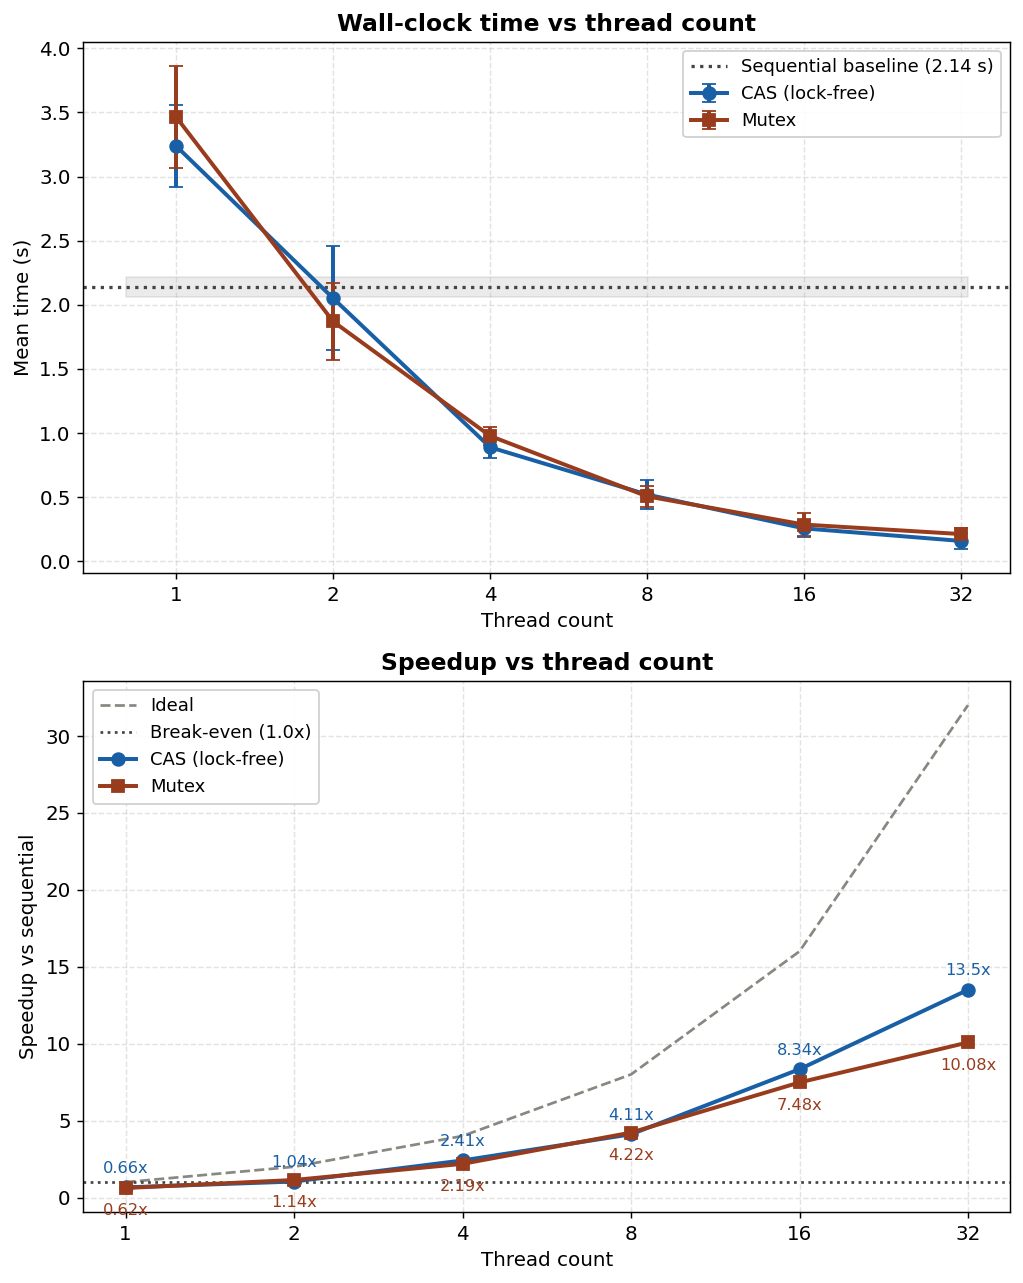
\includegraphics[width=0.4\textwidth]{exp1_thread_scaling.png}
    \caption{Experiment 1: Thread Scaling — CAS vs Mutex (10M table, 50\% load, Random keys)}
    \label{fig:exp1}
\end{figure}

\textbf{Analysis.} At one thread both parallel backends are
\emph{slower} than the pure sequential baseline (CAS 0.66$\times$,
mutex 0.62$\times$) because every slot access pays an atomic
load/CAS or a lock acquire that the sequential code does not. The
scaling curves diverge from 4 threads onward: CAS tracks close to
linear (4.11$\times$ at 8 threads, 8.34$\times$ at 16, 13.5$\times$
at 32), while mutex stays close to CAS through 8 threads, pulls
ahead briefly at 4 threads (2.19 vs 2.41 is within measurement
noise on our variance), and then falls behind at 16 and 32 threads
(7.48 vs 8.34; 10.08 vs 13.50). We learn that mutex overhead is
roughly a \emph{constant} fraction of CAS overhead up to the point
where lock cache lines begin to bounce between cores; above that
point the lock's coherence traffic scales with core count while
CAS traffic scales only with genuine contention. Under conditions
where contention is low \emph{and} the thread count stays under
$\sim$8, a practitioner would see almost no advantage from CAS;
above 16 threads the CAS advantage is decisive.

\subsection{Experiment 2: Key distribution and contention}
Configuration: $C = 10^7$, 16 threads, linear probing, load 0.5.

\begin{table}[h]
\centering
\scriptsize
\begin{tabular}{llrrr}
\toprule
Key dist & Backend & Mean (s) & Std & Speedup \\
\midrule
Sequential & Seq.\ baseline & 3.19051 & 0.179 & 1.00 \\
Sequential & CAS (16T)      & 0.29612 & 0.064 & 10.77 \\
Sequential & Mutex (16T)    & 0.29681 & 0.074 & 10.75 \\
Random     & Seq.\ baseline & 2.29230 & 0.075 & 1.00 \\
Random     & CAS (16T)      & 0.28882 & 0.072 & 7.94 \\
Random     & Mutex (16T)    & 0.34082 & 0.038 & 6.73 \\
Zipf       & Seq.\ baseline & 1.43740 & 0.045 & 1.00 \\
Zipf       & CAS (16T)      & 0.18765 & 0.013 & 7.66 \\
Zipf       & Mutex (16T)    & 0.14345 & 0.019 & 10.02 \\
\bottomrule
\end{tabular}
\caption{Experiment 2: effect of key distribution.}
\label{tab:e2}
\end{table}

\begin{figure}[h]
    \centering
    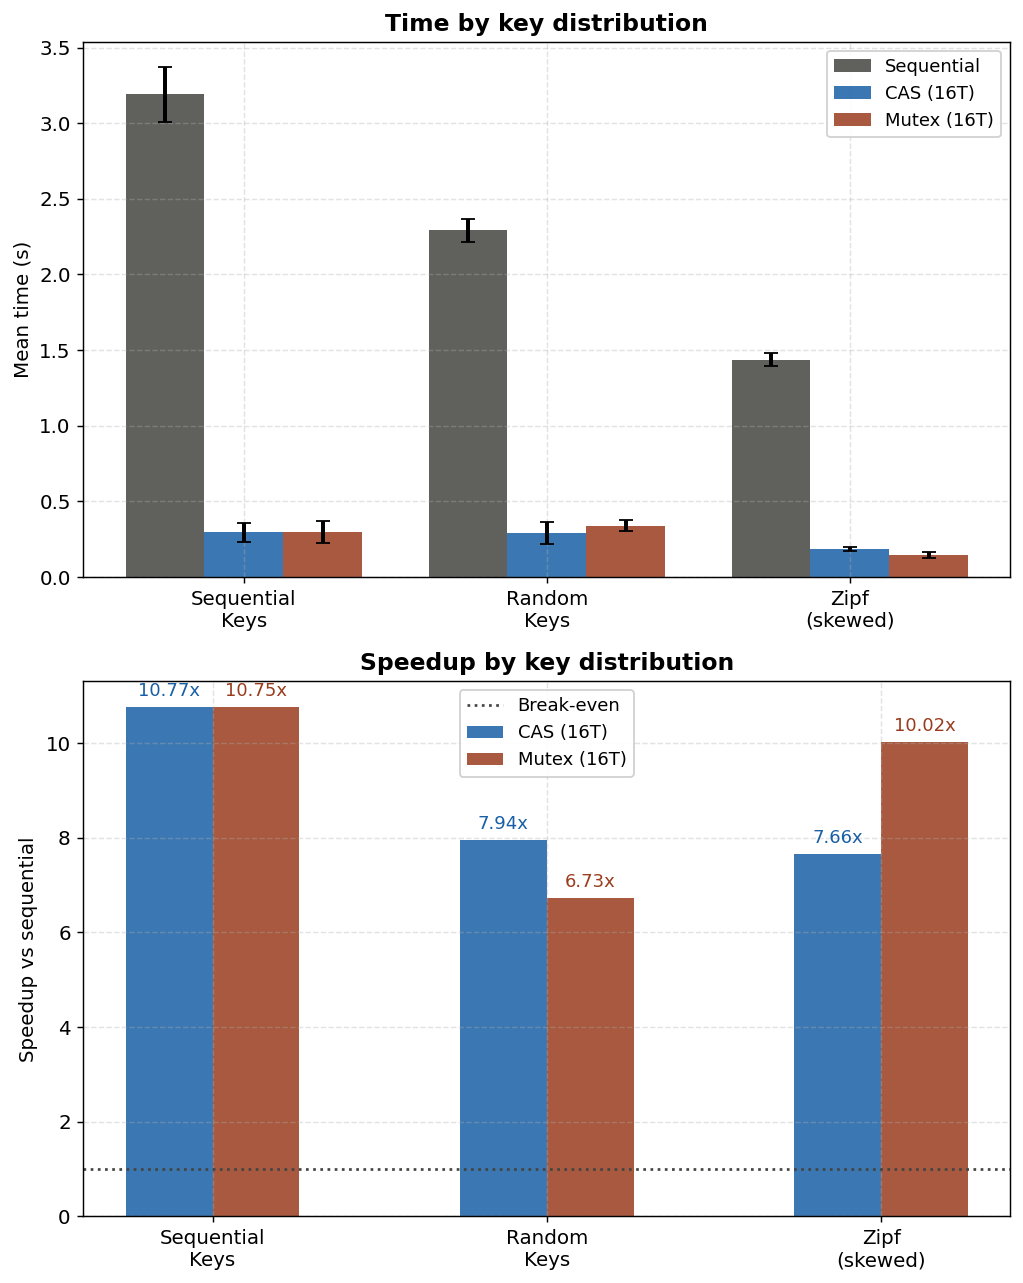
\includegraphics[width=0.4\textwidth]{exp2_key_distribution.png}
    \caption{Experiment 2: Key Distribution and Contention (10M table, 50\% load, 16 threads)}
    \label{fig:exp2}
\end{figure}

\textbf{Analysis.} Sequential keys give the largest speedup for
both backends (10.77$\times$ CAS, 10.75$\times$ mutex) because probe
collisions are rare---each new key hashes to a fresh slot and the
synchronization path is almost always uncontended. Random keys
introduce moderate collision pressure and CAS pulls ahead of mutex
(7.94 vs.\ 6.73). The Zipf result is the most interesting: the
\emph{mutex} backend beats CAS here (10.02 vs.\ 7.66), reversing
the pattern of every other experiment. The reason is that the
sequential baseline's own runtime collapses under Zipf (1.44~s
vs.\ 2.29~s on random), because sequential code revisits the same
few hot cache lines and hits them in L1; the speedup ratio is
therefore measured against a \emph{faster} denominator. Absolute
time still favours mutex by 0.187~s vs.\ 0.143~s, which we
attribute to CAS retry storms on the handful of hot slots: when
many threads race on the same key, every failed CAS forces a
retry, whereas the mutex path simply serialises. Under the
condition of extreme contention (few hot keys, many threads),
blocking synchronization can out-perform lock-free retry because
retries waste memory bandwidth while blocking at least releases
the core. We learn that ``lock-free is always better'' is too
strong a conclusion; the right answer depends on the contention
distribution.

\subsection{Experiment 3: Load factor $\times$ probing strategy}
Configuration: $C = 10^7$, 8 threads CAS, random keys.

\begin{table}[h]
\centering
\scriptsize
\begin{tabular}{rllrr}
\toprule
Load & Probing & Backend & Mean (s) & Speedup \\
\midrule
50\% & Linear    & Seq. & 2.65885 & 1.00 \\
50\% & Linear    & CAS  & 0.78705 & 3.38 \\
50\% & Quadratic & Seq. & 2.37526 & 1.00 \\
50\% & Quadratic & CAS  & 0.47034 & 5.05 \\
70\% & Linear    & Seq. & 3.65749 & 1.00 \\
70\% & Linear    & CAS  & 1.18382 & 3.09 \\
70\% & Quadratic & Seq. & 3.61477 & 1.00 \\
70\% & Quadratic & CAS  & 0.75888 & 4.76 \\
85\% & Linear    & Seq. & 5.33811 & 1.00 \\
85\% & Linear    & CAS  & 1.22026 & 4.37 \\
85\% & Quadratic & Seq. & 4.56212 & 1.00 \\
85\% & Quadratic & CAS  & 1.93907 & 2.35 \\
95\% & Linear    & Seq. & 6.87051 & 1.00 \\
95\% & Linear    & CAS  & 2.55534 & 2.69 \\
95\% & Quadratic & Seq. & 5.63551 & 1.00 \\
95\% & Quadratic & CAS  & 3.04324 & 1.85 \\
\bottomrule
\end{tabular}
\caption{Experiment 3: linear vs.\ quadratic probing at varying load
factors (CAS backend, 8 threads).}
\label{tab:e3}
\end{table}

\begin{figure}[h]
    \centering
    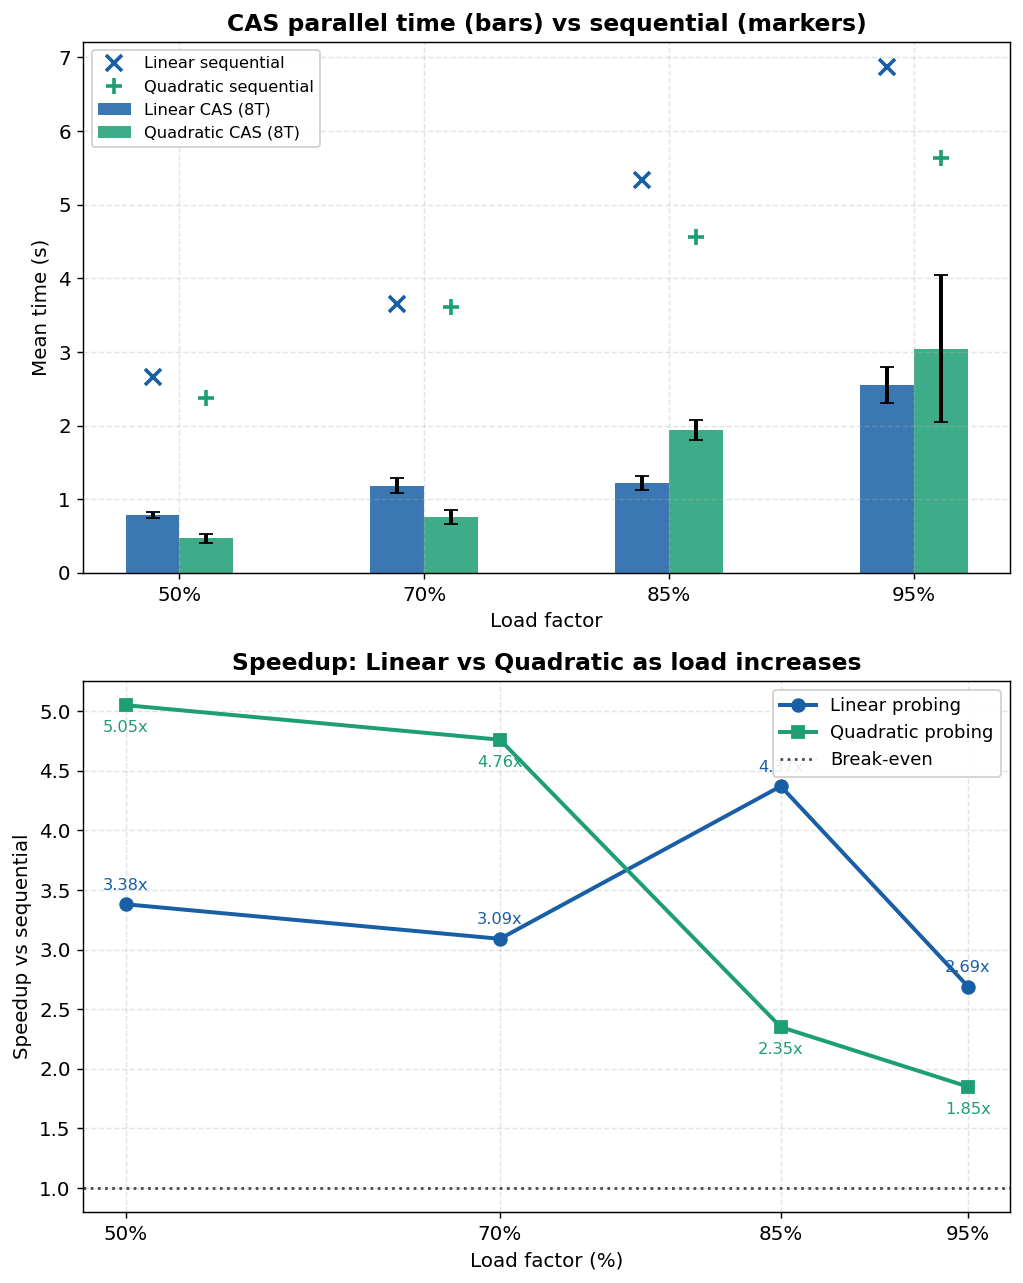
\includegraphics[width=0.4\textwidth]{exp3_probing_load.png}
    \caption{Experiment 3: Linear vs Quadratic Probing at Varying Load Factors (10M table, 8T CAS)}
    \label{fig:exp3}
\end{figure}

\textbf{Analysis.} At low load (50--70\%) quadratic probing is the
clear winner: 5.05$\times$ vs.\ 3.38$\times$ at 50\%, and
4.76$\times$ vs.\ 3.09$\times$ at 70\%. This is because quadratic
probing breaks primary clustering, so the expected probe length is
shorter and each failed probe no longer crowds the next thread's
hash target. At high load (85--95\%) the ordering inverts:
linear wins 4.37$\times$ vs.\ 2.35$\times$ at 85\% and
2.69$\times$ vs.\ 1.85$\times$ at 95\%. Two effects drive this
crossover. First, once the table is nearly full, quadratic
probing's stride of $i^2$ jumps between distant cache lines on
every attempt, while linear probing streams through consecutive
lines---quadratic turns every probe into a cache miss. Second,
quadratic probing does not cover all slots in a table of arbitrary
size, so under near-full conditions it can require many more
attempts to find a free slot. We learn that the choice of probing
strategy is not simply ``quadratic is better because it avoids
clustering''---the locality advantage of linear probing dominates
above $\alpha \approx 0.8$.

\subsection{Experiment 4: Table size and cache effects}
Configuration: 8 threads CAS, linear probing, random keys, load 0.5.

\begin{table}[h]
\centering
\scriptsize
\begin{tabular}{lllrr}
\toprule
Size & Backend & Mean (s) & Mops/s & Speedup \\
\midrule
100K & Seq.\ baseline & 0.01700 & 2.94 & 1.00 \\
100K & CAS (8T)       & 0.00865 & 5.78 & 1.97 \\
1M   & Seq.\ baseline & 0.35984 & 1.39 & 1.00 \\
1M   & CAS (8T)       & 0.09313 & 5.37 & 3.86 \\
10M  & Seq.\ baseline & 2.63535 & 1.90 & 1.00 \\
10M  & CAS (8T)       & 0.51185 & 9.77 & 5.15 \\
50M  & Seq.\ baseline & 12.6905 & 1.97 & 1.00 \\
50M  & CAS (8T)       & 2.79183 & 8.95 & 4.55 \\
\bottomrule
\end{tabular}
\caption{Experiment 4: throughput vs.\ table size.}
\label{tab:e4}
\end{table}

\begin{figure}[h]
    \centering
    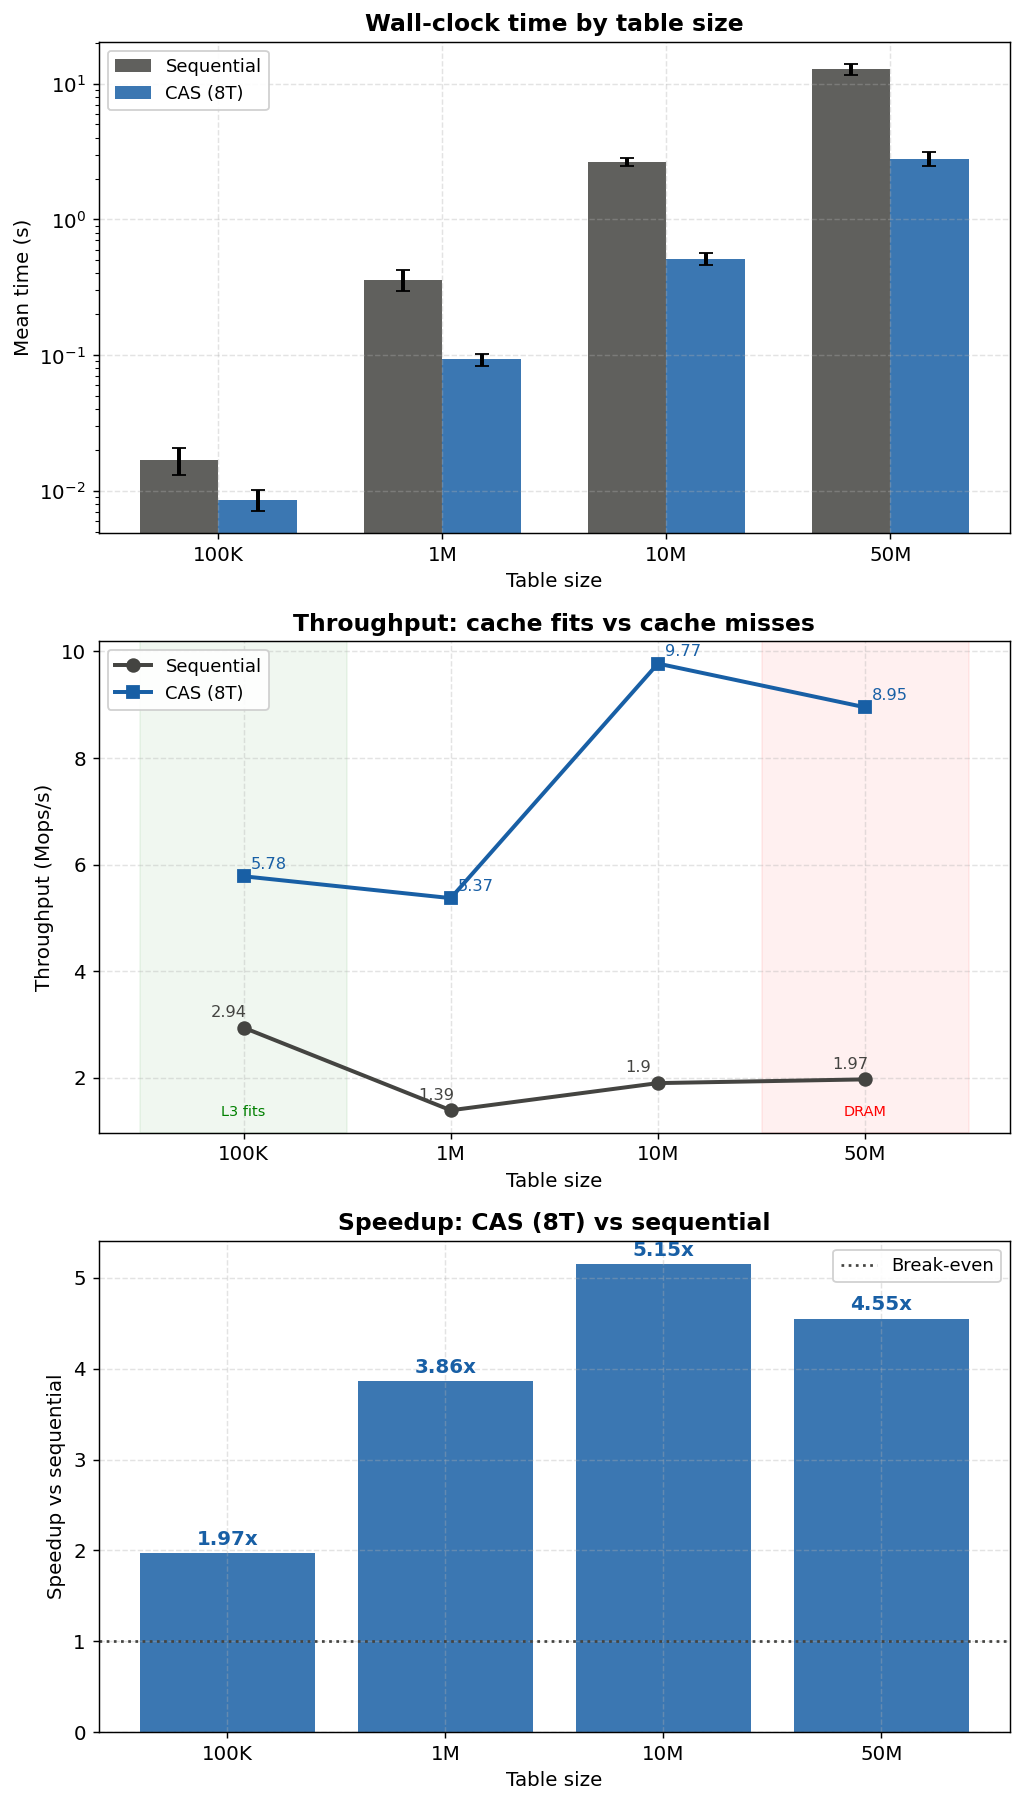
\includegraphics[width=0.4\textwidth]{exp4_table_size_cache.png}
    \caption{Experiment 4: Table Size and Cache Effects (8T CAS, Linear probing, 50\% load)}
    \label{fig:exp4}
\end{figure}

\textbf{Analysis.} The CAS speedup grows with table size up to the
LLC boundary and then declines beyond it. At 100K slots the entire
working set fits in L2 cache; thread launch and batch-scheduling
overhead dominate, limiting speedup to 1.97$\times$ on 8 threads
(ideal would be 8$\times$). At 1M (8~MB of slot data) and 10M
(80~MB), the sequential baseline becomes DRAM-bound, so adding
threads pays not only for parallel compute but for parallel memory
issue; speedup climbs to 5.15$\times$ at 10M. At 50M (400~MB,
comfortably larger than any CPU cache) the speedup drops back to
4.55$\times$ because the aggregate DRAM bandwidth of the socket
becomes the bottleneck---adding more threads cannot purchase more
memory controllers. The absolute throughput peak of 9.77~Mops/s at
10M is consistent with a memory-bandwidth-bound regime. Under
the condition of tiny working sets (fits in L1/L2), a practitioner
should \emph{not} expect linear scaling and should question
whether parallelisation is worthwhile at all; the answer is
``only if you are already DRAM-bound''.

\section{Conclusions}
Under identical storage and probing, the CAS backend scales
to 13.5$\times$ on 32 threads on uniform-random workloads, while the
per-slot mutex backend reaches 10.08$\times$; the CAS advantage is
small below 8 threads and grows once lock cache lines begin to bounce.

The choice of probing strategy reverses with load factor:
quadratic probing wins at $\alpha \le 0.7$ (up to 5.05$\times$ vs.\
3.38$\times$ at 50\%) because it defeats primary clustering, but
linear probing wins at $\alpha \ge 0.85$ (4.37$\times$ vs.\
2.35$\times$ at 85\%) because its sequential memory access pattern
survives near-full tables that break quadratic locality.

Lock-free is not universally better: under Zipf skew at 16
threads the mutex backend out-performs CAS (10.02$\times$ vs.\
7.66$\times$) because repeated CAS retries on a handful of hot slots
waste memory bandwidth, whereas blocking synchronisation serialises
cleanly. The right synchronisation discipline depends on the
contention distribution of the workload.

\begin{thebibliography}{9}

\bibitem{xue2025global}
Y.~Xue and R.~Marcus.
\newblock Global hash tables strike back! An analysis of parallel
GROUP BY aggregation.
\newblock \emph{arXiv preprint arXiv:2505.04153}, 2025.

\bibitem{tripathy2021numa}
A.~Tripathy and O.~Green.
\newblock Scalable hash table for NUMA systems.
\newblock \emph{arXiv preprint arXiv:2104.00792}, 2021.

\bibitem{areias2025chaining}
M.~Areias, R.~Rocha, and collaborators.
\newblock Performance evaluation of separate chaining for concurrent
hash maps.
\newblock \emph{Mathematics}, 13(17):2820, 2025.

\bibitem{liao2023cuckoo}
J.~Liao et~al.
\newblock Lock-free bucketized cuckoo hashing.
\newblock In \emph{Euro-Par 2023: Parallel Processing}, Lecture Notes in
Computer Science, pages 393--407. Springer, 2023.

\bibitem{singh2025pop}
A.~Singh et~al.
\newblock Publish on ping: Efficient and reliable memory reclamation via
signals.
\newblock \emph{arXiv preprint arXiv:2501.04250}, 2025.

\bibitem{kim2024epic}
J.~Kim et~al.
\newblock Are your epochs too epic? Batch free can be harmful.
\newblock In \emph{Proceedings of the 29th ACM SIGPLAN Symposium on
Principles and Practice of Parallel Programming (PPoPP)}, pages
nil, 2024.

\bibitem{sheffi2022era}
G.~Sheffi and E.~Petrank.
\newblock The ERA theorem for safe memory reclamation.
\newblock \emph{arXiv preprint arXiv:2211.04351}, 2022.

\end{thebibliography}

\end{document}
